
		 \section{Eigenwerte / Eigenvektoren}   
		 Ein Vektor $\vec{v}$ heisst Eigenvektor der $n \times n$ Matrix A zum \\
		 Eigenwert $\lambda$, wenn 
		$$A \vec{v} = \lambda \vec{v} \quad \text{und} \quad \vec{v \neq 0}$$
		\\
		\textbf{Eigenschaften}\\
		\begin{tabular}{ll}
		$\bullet$ & Ein Eigenvektor $\vec{v}$ wird durch die Matrix A nur gestreckt \\
		& (Streckungsfaktor $\lambda$) \\
		$\bullet$ & Es gibt maximal n verschiedene Eigenwerte $\lambda$ \\
		$\bullet$ & Zu jedem Eigenwert gibt es unendlich viele Eigenvektoren \\
		\end{tabular}		 
		 
	 
	 
		 \textbf{Eigenwerte und Eigenvektoren finden} \\
		 \begin{tabular}{ll}
		1. & Eigenwertproblem: $A \textcolor{red}{\vec{v}} = \textcolor{red}{\lambda \vec{v}}$ $\Rightarrow$  $(A - \lambda E) \vec{v} = 0$  \\
		2. & Charakteristische Gleichung: $\det(A -  \textcolor{red}{\lambda} E) = 0$ \\
		3. & Berechnung der Eigenwerte \textcolor{red}{$\lambda_i$} als Lösungen der \\
		& charakteristischen Gleichung \\
		4. & Berechnung der Eigenvektoren \textcolor{red}{$\vec{v_i}$} mittels Gauss-Algorithmus: \\
		& $(A - \lambda_i E) \vec{v_i} = 0$ \\
		5. & Resultat kontrollieren: $A \vec{v_i} = \lambda_i \vec{v_i}$ \\
		\\
		\end{tabular}		 
		
		
		Hinweis: Wenn $AA^t$ oder $A^tA$	eine Zeile und Spalte mit nur\\
		einem Zahleneintrag enthalten, so ist die Zahl ein Eigenwert zum \\
		zugehörigen Standardbasisvektor. \\
		Die weiteren EW und EV können ohne diese Zeile/Spalte berechnet werden!	   
			
			
			\subsection{Eigenschaften der Matrix A bzgl. Eigenwerte}
			\begin{tabular}{ll}
			$\bullet$ & Spur($A$) = Spur($A'$) = Summe der Eigenwerte von $A$ \\
			$\bullet$ & $\det(A) = \det(A')$ = Produkt aller Eigenwerte von $A$\\
			\\
			\end{tabular}
			
			\begin{minipage}{0.35\linewidth}
			$AA^t = \begin{pmatrix} 2 & 0 & -2 \\ 0 & 9 & 0 \\ -2 & 0 & 2 \end{pmatrix}$ \\
			\\
			$A_0 = \begin{pmatrix}2 & -2 \\ -2 & 2 \end{pmatrix}$						
			
			\end{minipage}	
			\hfill
			\begin{minipage}{0.55\linewidth}
			
			Aus $AA^t$ kann man $\lambda = 9$ direkt ablesen. \\
			
			Daraus folgt: $\vec{v_{\lambda}} = \begin{pmatrix} 0 \\ 1 \\ 0 \end{pmatrix}$	
			\end{minipage}					   
		   
		   
		   
		   
		   
				\subsubsection{Beispiel Eigenwerte und Eigenvektoren berechnen}
		 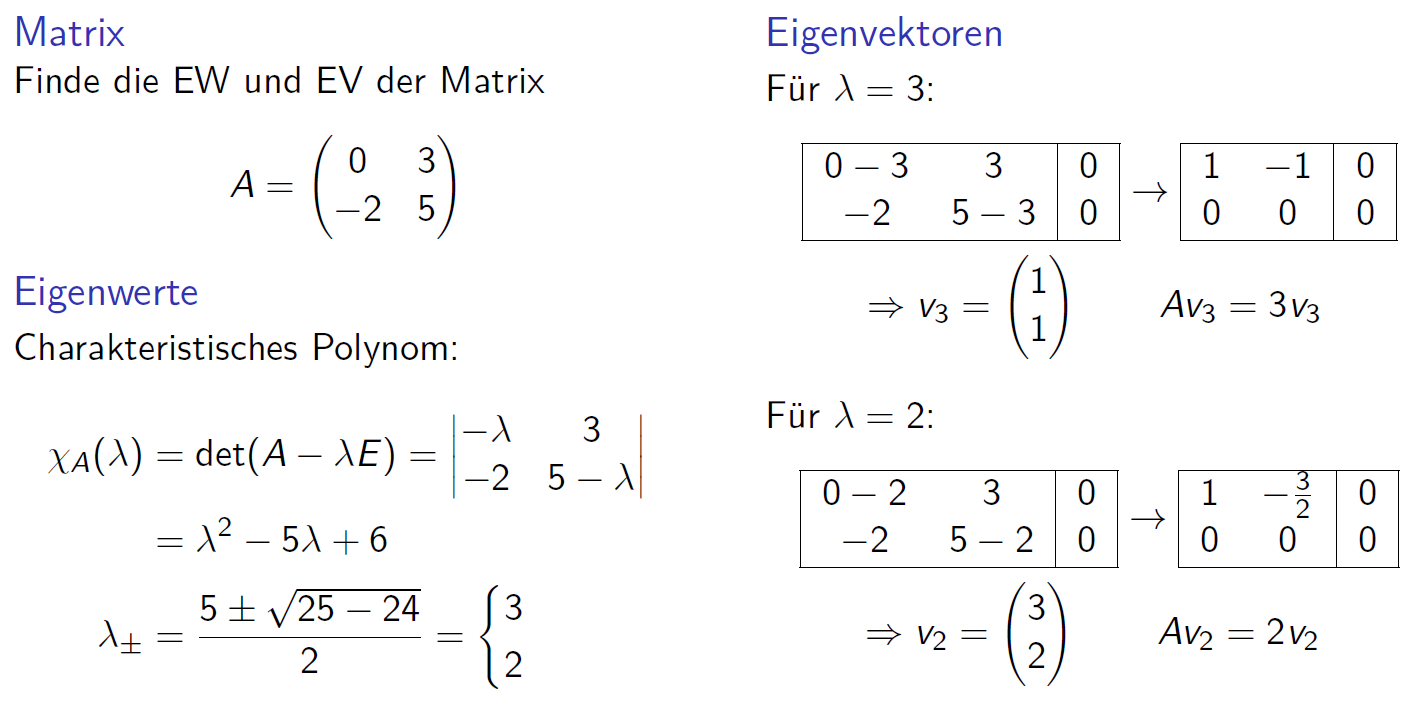
\includegraphics[width=0.85\linewidth]{Bilder/eigenwerte-eigenvektoren} \\
		 
			\textbf{Rechenregeln für Eigenwerte}
			$\frac{1}{\lambda} = \lambda - 1$ \\		 
		 
		 
		 
		 
		 
		 
		 
		 
		 
		 
		   \subsection{Diagonalisierung einer Matrix}
			Mit Diagonalmatritzen kann man einfach rechnen \\	
			\\
			\textbf{Eine Matrix ist diagonalisierbar, wenn:} \\
			\begin{tabular}{ll}
			$\bullet$ & Die Matrix symmetrisch ist , also $A = A^t$\\
			$\bullet$ & \textbf{Eine Basis aus Eigenvektoren existiert} \\
			\end{tabular}				    
			
			\subsubsection{Vorgehen Matrix diagonalisieren} 
		 \begin{tabular}{ll}
		1. & Eigenbasis $C$ aus n linear unabh. Eigenvektoren finden  \\
		& Spalten von $C$ sind Eigenvektoren\\
		2. & Basis-Transformationsmatrix $T$ berechnen \\
		& $T = C^{-1}$ $\rightarrow$ Matrix aus Eigenvektoren invertieren \\
		3. & Diagonalisierte Matrix $A'$ berechnen \\
		& $A' = T A T^{-1}$ $\rightarrow$ $A$' enhält Eigenwerte auf Diagonalen \\
		\end{tabular}		 
		 
		  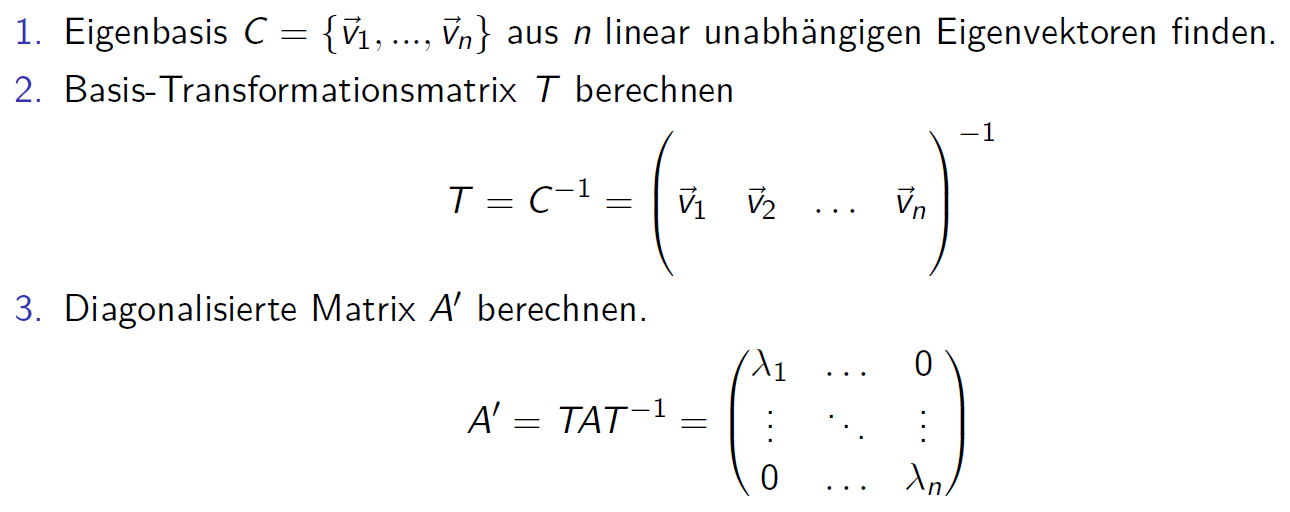
\includegraphics[width=0.7\linewidth]{Bilder/matrix-diagonalisieren} \\ 
			
			
			

			\subsubsection{Transformationsmatrix $T$; Eigenbasis $C$}
			\begin{tabular}{ll}
			$\bullet$ & Die Eigenbasisis-Matrix $C$ enthält in ihren Spalten die \\
			& Eigenvektoren der Matrix $A$ (Anfangsmatrix) \\
			$\bullet$ & Die Transformationsmatrix $T$ ist die Inverse von $C$ \\
			\end{tabular}
			
			\subsubsection{Spezialfall Symmetrische Matrix diagonalisieren}
		    
			Die Eigenvektoren einer symmetischen Matrix sind orthagonal \\
		   
		   
		   \subsection{Singulärwertzerlegung (SVD)}
			Eine $m \times n$ Matrix $A$ wird zerlegt in zwei orthagonale Matritzen und eine Diagonalmatrix \\
			$A = U \, \Sigma \, V^t$	 \\	  
			\\
			\begin{tabular}{ll}
			$U$ & orthagonale $m \times m$ Matrix  ($U$ diagonalisiert $AA^t$)\\
			$V$ & orthagonale $n \times n$ Matrix ($V$ diagonalisiert $A^tA$)\\
			$V^t$ & Transponierte von $U$ \\
			$\Sigma$ & Diagnonalmatrix mit $r$ Singulärwerten $\sigma_0$ bis $\sigma_r$ \\
			\end{tabular}			 
		   
		   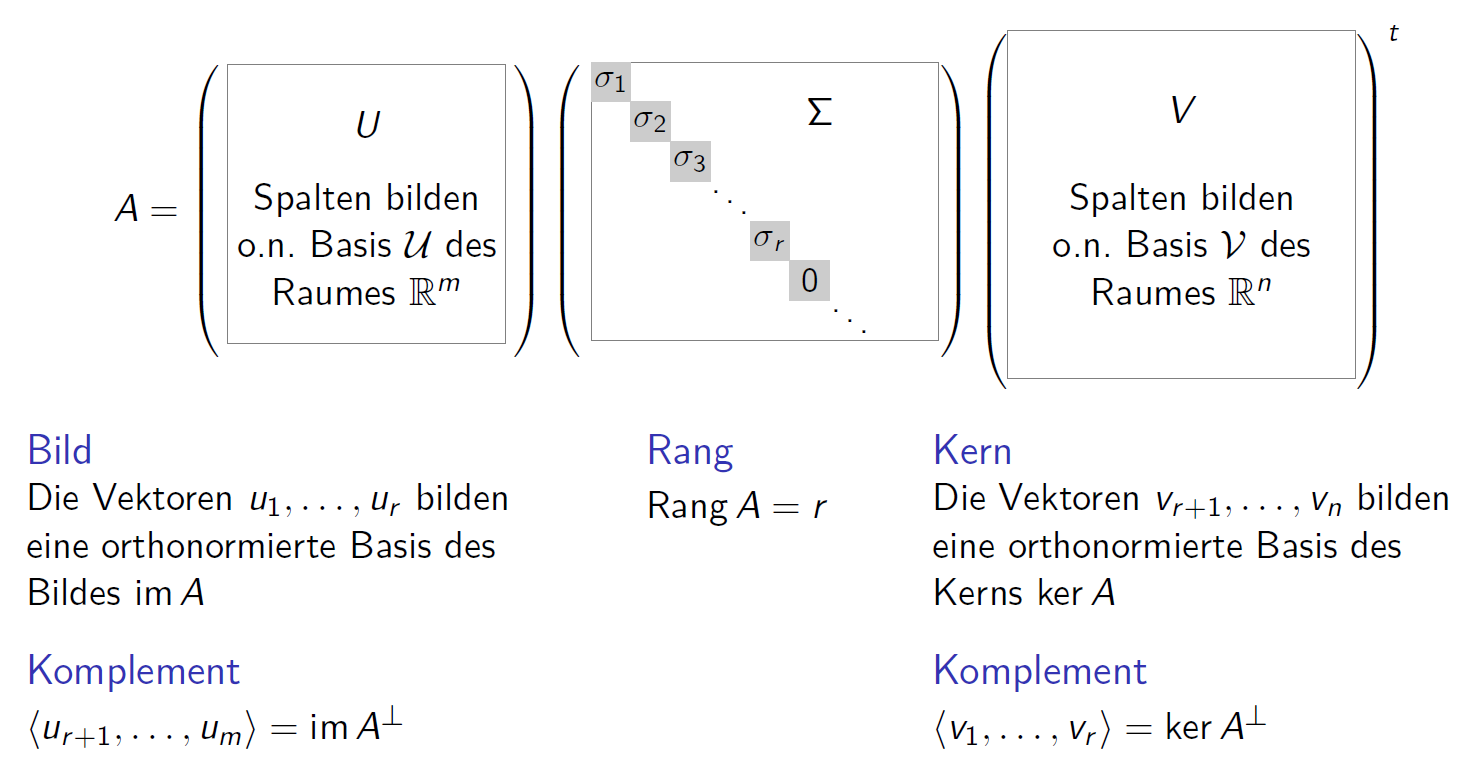
\includegraphics[width=0.65\linewidth]{Bilder/SVD} \\
		   
		   
			
		   
		   \subsubsection{Vorgehen Singulärwertzerlegung}
		   \begin{tabular}{ll}
		   1. & $AA^t$ und $A^tA$ berechnen \\
		   2. & Eigenwerte von $AA^t$ oder $A^tA$ berechnen (EW identisch) \\
		   3. & Eigenwerte der Grösse nach sortieren: $\sigma_1 \geq \sigma_2 \geq ... \geq \sigma_r \geq 0$\\
		   4. & $V$ = auf Länge 1 normierte Eigenvektoren von $A^tA$ \\
		   5. & $U$ = Spalten $u_i$ mit $u_i = \frac{A v_i}{\vert A v_i \vert}$ \\
		   6. & Singulärwerte bestimmen: $\sigma_i = \sqrt{\lambda_i}$ und Matrix $\Sigma$ füllen \\
		   7. & Kontrolle mit $A = U \, \Sigma \, V^t$ \\
		   \end{tabular}
		   
		   
			
	
			
			
		   \subsection{Pseudoinverse}
			\textbf{Die Pseudoinverse löst  Gleichungssysteme mit der Lösung minimaler Länge}		\\   
			$\vert x \vert$ ist minimal \\
		   
		     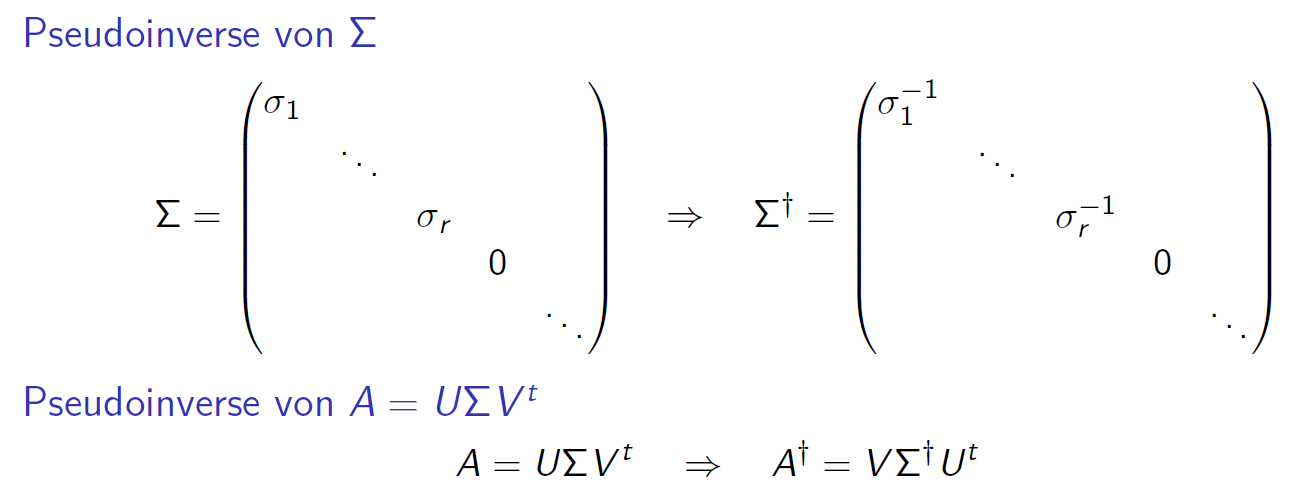
\includegraphics[width=0.8\linewidth]{Bilder/pseudoinverse} \\
		     
		    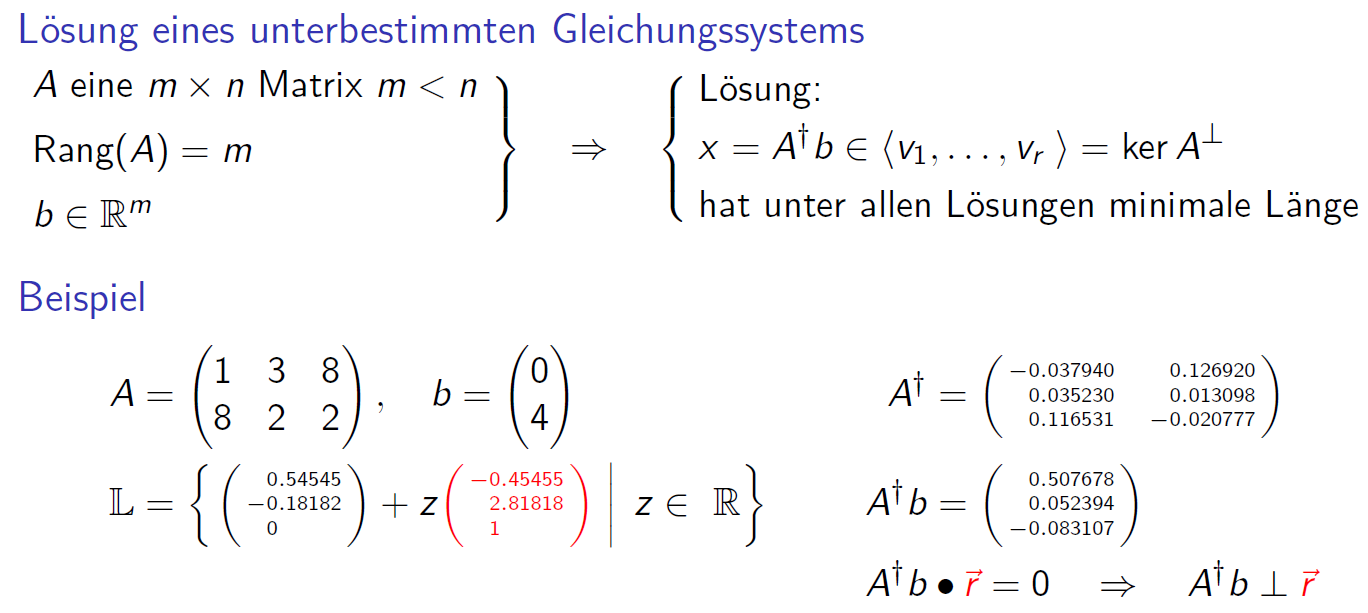
\includegraphics[width=0.8\linewidth]{Bilder/pseudoinverse2} \\
		    
		    
		    